
\section{Modèle avec composantes IT et WR (FIRE-IT-WR)}
\subsection{Question 2.2.1}
Avec la composante WR, nous effectuons la recherche des témoignes. 2 paramètres sont introduits dans cette partie sont nBF (facteur de branchement) et nRL (seuil de longueur de référence). Lors de la sélection d'un fournisseur, le consommateur envoie une requête à nBF de ses voisins les plus susceptibles de connaître le fournisseur dont on cherche une valeur de confiance. La sélection parmi les voisins s'effectue avec la mesure de distance qui le sépare du fournisseur. Les agents ayant reçu cette requête renvoie, soit les notes du fournisseur s'ils ont effectivement eu une interaction avec, soit une liste de leurs voisins susceptibles de le connaître. Ainsi cette boucle s'itère jusqu'à ce que la longueur de la chaîne atteigne nRL ou jusqu'à ce que le consommateur ait trouvé nBF témoins (c'est à dire nBF agents ayant eu une interaction avec le fournisseur).

\begin{algorithm}[H]
\caption{WR-Evaluation}
\begin{algorithmic} 
\STATE chainLength $\leftarrow$ 0
\STATE witnessNb $\leftarrow$ 0
\STATE ratingsList $\leftarrow$ [ ]
\STATE acquaintances $\leftarrow$ [ ]
\WHILE{acquaintances.length < nbF}
\STATE acquaintances $\leftarrow$ likelyAcquaintances
\ENDWHILE
\WHILE{witnessNb < nBF and chain < nRL}
\STATE chain ++
\FORALL{Provider p in acquaintances}
\STATE acquaintances.remove(self)
\IF {matchingRatingsFound}
\STATE ratingsList $\leftarrow$ ratingList $\cup$ ratings
\STATE witnessNb ++
\ELSE
\STATE acquaintances $\leftarrow$ acquaintances $\cup$ listOFnewAcquaintances
\ENDIF
\ENDFOR
\ENDWHILE

\STATE RW $\leftarrow$ ratingsList
\STATE TV $\leftarrow$ getTrustValue (WR)
	
\end{algorithmic}
\end{algorithm}





Quand le consommateur reçoit les notes des témoins, il évalue ces notes et celles de sa base de données locale pour avoir une valeur de confiance avec l'ensemble des informations qu'il possède. Nous avons donc du modifier la méthode getTValue pour la rendre générique.

\begin{algorithm}[H]
\caption{get Trust Value}
\begin{algorithmic} 
\STATE t-value $\leftarrow$ 0
\STATE weightSum $\leftarrow$ 0
\STATE r-ab $\leftarrow$ $\empty$
\FORALL{k in every components of t-model}
    \STATE r-ab $\leftarrow$ get-rates-for b from component k
    \STATE tk $\leftarrow$ get-t-value-by-component r-ab
    \STATE reliability $\leftarrow$ get-reliability for component k
    \STATE w $\leftarrow$ get-component's coefficient * reliability
    \STATE t-value $\leftarrow$ t-value + component's weight * tk
    \STATE weight-sum $\leftarrow$ weight-sum + w
\ENDFOR
\STATE t-value $\leftarrow$ t-value / weight-sum
\RETURN t-value
\end{algorithmic}
\end{algorithm}

où getTValueByComponent correspond à :

\begin{algorithm}[H]
\caption{get Trust Value for b by Component k}
\begin{algorithmic} 
\STATE t-value $\leftarrow$ 0
\STATE weightSum $\leftarrow$ 0

\IF{k = IT}
\STATE r-ab $\leftarrow$ self.getRates(b)
\ENDIF
\IF{k = WR}
\STATE r-ab $\leftarrow$ wr-evaluation(b)
\ENDIF
\IF{k = CR}
\STATE r-ab $\leftarrow$ b.receivedRatings
\ENDIF

\FORALL{r in r-ab}
\STATE ug $\leftarrow$ r[v] * 10
\STATE ug $\leftarrow$ ug + $\delta$UG
\STATE v $\leftarrow$ ug / 10
\STATE weight $\leftarrow$ $\frac{\exp{ (-1*this.tick-r[i]) }}{\lambda}$
\STATE weightSum $\leftarrow$ weightSum + weight
\STATE t-value $\leftarrow$ t-value + weight * v
\ENDFOR
\STATE t-value $\leftarrow$ t-value / weightSum
\RETURN t-value
\end{algorithmic}
\end{algorithm}


$\delta$UG sera expliqué dans la partie 4.2.

La méthode getReliability a également été modifiée de la même manière.

\subsection{Question 2.2.2}
Nous avons du modifier quelques paramètres afin d'obtenir une simulation acceptable. Lorsque un groupe de consommateurs avec le composant WR (IT-WR ou IT-WR-CR) est présent, nous avons remarqué que le lancement était beaucoup trop lent. N'ayant pas pu régler ce problème dans les délais, nous devions diminuer soit le nombre de consommateurs par groupe (Nc) soit la longueur des chaînes de recherches de témoins (nRL). C'est finalement cette dernière qui a été diminuée. 

\subsection{Question 2.2.3}
\begin{figure}[H]
    \centering
    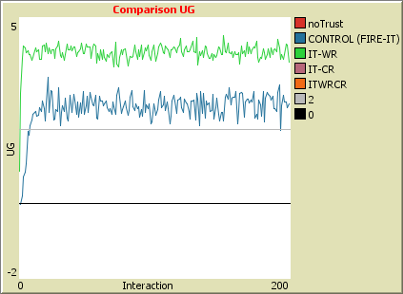
\includegraphics[width=0.8\textwidth]{images/ITvsITWR.png}
    \caption{Reproduction de la figure 9}
    \label{fig:itvswr}
\end{figure}

Comme expliqué ci-dessus, le temps d'exécution était très grand même après l'optimisation du code. Nous avons, entre autres, crée un attribut \texttt{neighbours} propre à chaque agents afin de ne pas lancer la recherche de voisins plusieurs fois. Malgré cet inconvénient, et le changement de paramètres liés, nous avons quand même un résultat assez convenable. \newline La présence du composant WR permet aux agents d'accéder à des informations concernant un fournisseur plus rapidement.